\subsection{Comparação entre Controlador Proporcional, PID com Dados Iniciais e PID Ajustado}
Este fragmento apresenta uma análise comparativa dos desempenhos de três diferentes configurações de controladores: Proporcional, PID com valores iniciais e PID ajustado, enfocando suas respostas em termos de estabilidade, tempo de resposta e precisão no estado estacionário.



\begin{figure}[H]
    \centering
    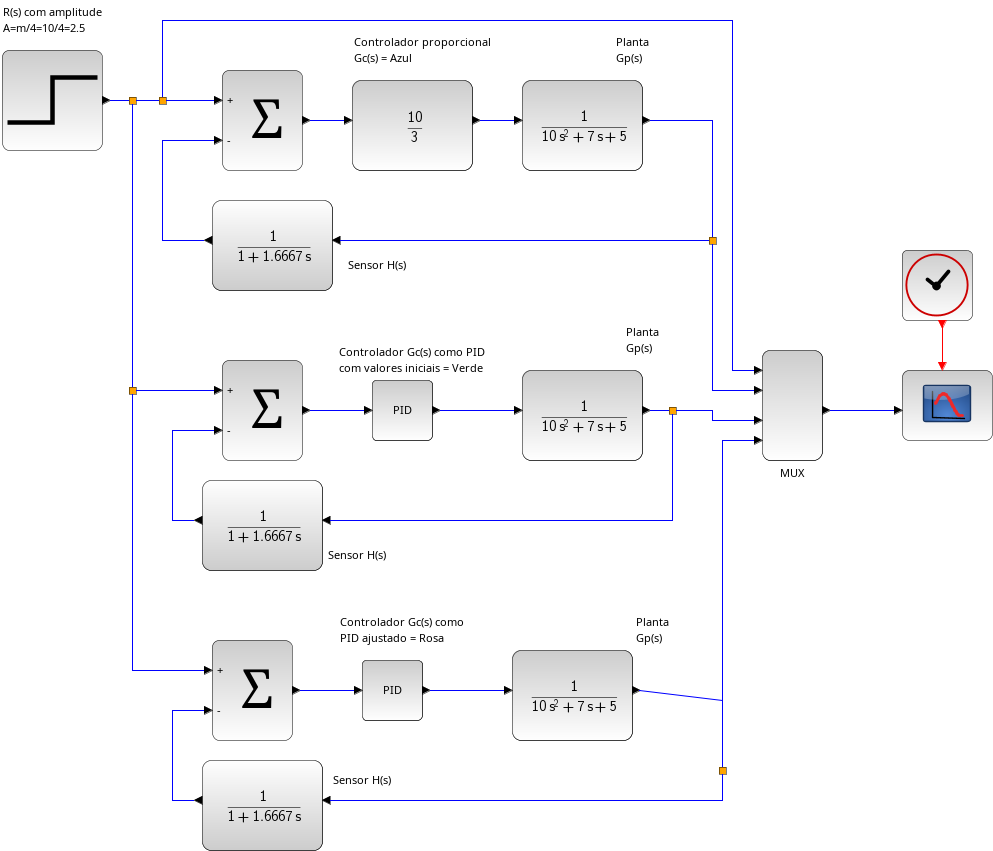
\includegraphics[width=0.8\textwidth]{6-atividade/assets/d/diagrama-comparacao-proporcional-pid-pid-ajustado.png}
    \caption{Diagrama de resposta do sistema com diferentes valores de \( K_p \).}
    \label{fig:diagrama-comparacao-proporcional-pid-pid-ajustado}
\end{figure}

\begin{figure}[H]
    \centering
    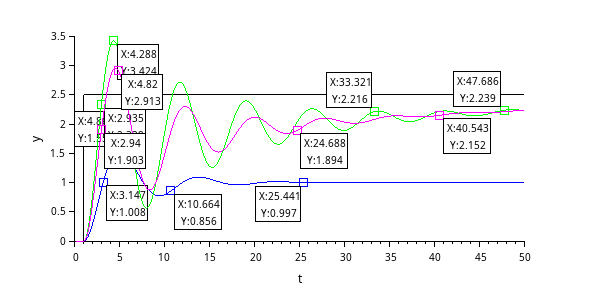
\includegraphics[width=0.8\textwidth]{6-atividade/assets/d/comparacao-proporcional-pid-pid-ajustado.png}
    \caption{Diagrama de resposta do sistema com diferentes valores de \( K_p \).}
    \label{fig:comparacao-proporcional-pid-pid-ajustado}
\end{figure}


\subsubsection{Análise dos Controladores}

\subsubsection{Controlador Proporcional (Azul)}
\textbf{Comportamento:} O controlador proporcional mostra uma rápida resposta inicial, mas não consegue eliminar o erro de estado estacionário, característica típica dos controladores proporcionais devido à ausência de ação integral.

\textbf{Estado Estacionário:} A resposta estabiliza-se abaixo do valor de referência, demonstrando a incapacidade de corrigir o erro de estado estacionário completamente.

\subsubsection{PID com Valores Iniciais (Verde)}
\textbf{Comportamento:} Exibe overshoot significativo e oscilações antes de estabilizar. A resposta rápida é seguida por uma correção mais intensa devido à ação integral.

\textbf{Estado Estacionário:} Atinge e mantém o valor desejado graças à componente integral, que ajusta o erro acumulado, assegurando que a saída final corresponda ao valor de referência.

\subsubsection{PID Ajustado (Rosa)}
\textbf{Comportamento:} A redução em \(K_p\) para 7.1664 amenizou o overshoot e proporcionou uma abordagem mais suave na resposta ao degrau. A resposta inicial menos agressiva indica um melhor equilíbrio entre as ações proporcional e integral.

\textbf{Estado Estacionário:} Alcança o estado estacionário com menos oscilações, refletindo uma melhoria na estabilidade geral do sistema. A ação integral ainda compensa o erro residual, garantindo equivalência ao valor do degrau.

\subsection{Conclusão e Implicações para o Ajuste de \(K_p\)}
Reduzir \(K_p\) a 80\% do valor inicial provou ser uma estratégia eficaz para melhorar a qualidade da resposta. Esta modificação suavizou a ação proporcional, permitindo que a integral operasse de forma mais eficaz, sem induzir instabilidade por overshoot excessivo.

\textbf{Considerações Adicionais:}
\begin{itemize}
    \item Uma redução ainda maior em \(K_p\) pode resultar em uma resposta excessivamente amortecida, tornando o sistema lento para alcançar o estado estacionário em condições de carga variável ou frente a perturbações externas.
    \item O ajuste fino de \(K_p\) deve ser ponderado cuidadosamente com base nas exigências específicas da aplicação e nas características desejadas da resposta do sistema.
\end{itemize}

Experimentar com diferentes valores de \(K_p\) em um ambiente controlado de simulação é recomendado para identificar o melhor conjunto de parâmetros que equilibram estabilidade e precisão.
